%
%                       This is a basic LaTeX Template
%                       for the Informatics Research Review

\documentclass[a4paper,11pt]{article}
% Add local fullpage and head macros
\usepackage{head,fullpage}     
% Add graphicx package with pdf flag (must use pdflatex)
\usepackage[pdftex]{graphicx}  
% Better support for URLs
\usepackage{url}
% Date formating
\usepackage{datetime}
% For Gantt chart
\usepackage{pgfgantt}
\usepackage{xcolor}
\usepackage[utf8]{inputenc}
\usepackage{subfig} 
\usepackage{caption}
\usepackage{placeins}

\addtolength{\skip\footins}{1em}
\captionsetup{justification=centering}
\newdateformat{monthyeardate}{%
  \monthname[\THEMONTH] \THEYEAR}

\parindent=0pt          %  Switch off indent of paragraphs 
\parskip=5pt            %  Put 5pt between each paragraph  
\Urlmuskip=0mu plus 1mu %  Better line breaks for URLs


%                       This section generates a title page
%                       Edit only the following three lines
%                       providing your exam number, 
%                       the general field of study you are considering
%                       for your review, and name of IRR tutor

\newcommand{\examnumber}{s1843212}
\newcommand{\field}{\vspace{0.2em} Developing an Application to\\ Introduce Parallel Task Scheduling}
\newcommand{\tutor}{Valentina Andries}
\newcommand{\supervisor}{Murray Cole}

\begin{document}
\begin{minipage}[b]{110mm}
        {\Huge\bf School of Informatics
        \vspace*{17mm}}
\end{minipage}
\hfill
\begin{minipage}[t]{40mm}               
        \makebox[40mm]{
        
\includegraphics[width=40mm]{crest.png}}
\end{minipage}
\par\noindent
    % Centre Title, and name
\vspace*{2cm}
\begin{center}
        \Large\bf Informatics Project Proposal \\
        \Large\bf \field
\end{center}
\vspace*{1.5cm}
\begin{center}
        \bf \examnumber\\
        \monthyeardate\today
\end{center}
\vspace*{5mm}

%
%                       Insert your abstract HERE
%                       
\begin{abstract}
    This project aims to develop an game-like application to introduce the concept and details parallel task scheduling to students. The report starts with backgrounds in parallel programming, providing the general scope, then describes the complexity of task graph scheduling problems, including all the variants to be included in the application. Afterwards, the design of the application is introduced, including ways of interaction, appearance of interface and selection of libraries. Finally, it briefly introduces the evaluation method, expected outcomes and planning of the project.
\end{abstract}

\vspace*{1cm}

\vspace*{3cm}
Date: \today

\vfill
{\bf Tutor:} \tutor\\
{\bf Supervisor:} \supervisor
\newpage

%                                               Through page and setup 
%                                               fancy headings
\setcounter{page}{1}                            % Set page number to 1
\footruleheight{1pt}
\headruleheight{1pt}
\lfoot{\small School of Informatics}
\lhead{Informatics Research Review}
\rhead{- \thepage}
\cfoot{}
\rfoot{Date: \date{\today}}
%
\tableofcontents                                % Makes Table of Contents

\section{Motivation}

Computing performance is highly demanded in IT industry and academic researches. For companies, they can easily acquire terabytes of user data, which requires massive computing resources to process timely. For researches in areas like physics, researchers rely on simulation to evaluate the behavior of models, which also requires more computing resource to have higher resolution. However, the speed of improvements in computing power of single processor core is slowing down. In this case, the developers have to rely on parallel computing to utilize more computing resources and to reduce the time cost to finish one job.

In parallel programming, a common practice is to divide a big job into several tasks with dependency. Typically, the tasks and dependencies will form a directed acyclic graph (DAG), which is called task graph\cite{Robert2011}. To have the job executed in a cluster, a task scheduler will use scheduling algorithms to assign each task in the task graph to processors in the given cluster. Different scheduling algorithms will lead to different assignments of tasks, resulting in different performance characteristics of the system, like delay and throughput. Therefore, it is beneficial for students to learn such algorithms 1) to understand the design and behavior of such scheduling frameworks; 2) to implement tasks that are more friendly for parallel execution and 3) to tweak or implement scheduling platforms according to engineering requirements.

\subsection{Problem Statement} \label{sec:prob}

As is described in previous section, algorithms are used for resource allocation of task graph. This process is called task graph scheduling. However, it is not easy to learn, mainly due to the variation of system configurations and algorithms, which will be introduced in detail in section \ref{sec:tgs}. For different combination of cluster model and scheduling algorithms, it leads to different steps in calculation, and for students, makes the algorithms more confusing to understand. Therefore, this project aims to develop an application to help the students to understand the issues in task graph scheduling and to learn the algorithms in a more interesting and interactive way.  Using this application, the students should be able 1) to try different allocation of tasks for various combination of models and task graphs, then see the execution results and 2) to simulate and verify the behavior of standard algorithms.

\subsection{Research Hypothesis and Objectives} \label{sec:obj}

As stated before, this project aims to help students learn scheduling algorithms better. It is hypothesized that using this application can provide solid learning outcomes and pleasant learning experience. To achieve better results, the design of application should provide strong feedback and satisfaction. Also, it should provide intuitive control logic to make it easier to use.

For variances in system models and scheduling algorithms, the application will include all of them if time allows. Otherwise, it should at least include some representative variances to provide a complete view of the problem.

In this project, the learning outcome will not be compared to that of traditional learning methods due to the limit of time and participants. In this case, it should typically provide a qualitative feedback on user experience and learning outcomes.

\subsection{Timeliness and Novelty}

For the content to be introduced, although some of the scheduling algorithms are invented tens of years before, they are still meaningful to learn and widely used in industrial practice, because parallel computing is gaining popularity to solve computation intensive problems. Many companies now rely on distributed computing frameworks like Hadoop and Spark for data processing, where YARN, a resource management system, is used to allocate computing tasks to processors. Task scheduling algorithms are important theory backgrounds in design of such systems. 

Secondly, although it is not common, it is a trend to use such applications or games to assist teaching in university education, since the volume of knowledge sometimes makes it hard for students to learn in limited time, while using such applications is promising to produce better learning outcomes. There seems to be no such projects related to task scheduling algorithms, so this project can propose a possible application of this teaching method in such area.

\subsection{Significance} \label{sec:sig}

Since this project is proposed for practical usage, the main significance is to help the students learn better about the algorithms and to possibly save time for tutors. It should also perform as a handy development and testing environment for graph task scheduling algorithms. As well as the details of algorithms, this application actually introduces the concept of scheduling, which is not only used in parallel programing tasks. Therefore, it can be useful to introduce similar concepts like database query planning or project management, with slight tweaks to the model. In addition, it can be considered an example implementation of game-like applications for teaching purpose on selected platforms and libraries. The design logic and implementation details can be referred by similar projects in the future.

\subsection{Feasibility}

To implement all the variances of model and algorithm with step-by-step introduction, it is estimated to take about 5-10k lines of pure code according to previous experience. Given a 2 month period excluding document writing and testing, it results in over 100 lines of code added per day, which seems feasible, but slightly challenging, considering there might be some reconstitution for projects in this size. For a basic working application, it is estimated to take less than 2k lines, reducing the production rate to less than 50 lines per day, which seems relatively easy.

\subsection{Beneficiaries}

As described in section \ref{sec:sig}, the direct beneficiaries are students learning and tutors teaching the task graph scheduling algorithms, but it could also be useful to teach similar concepts. In addition, the implementation details can be helpful as reference when anyone is building similar applications. 

\section{Background}

\subsection{Task Graph Scheduling} \label{sec:tgs}

\begin{figure}[htpb]
    \centering
    \subfloat[task graph]{ 
        \label{fig:graph}
        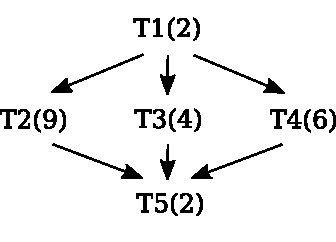
\includegraphics[width=0.3\columnwidth]{graph.pdf}
    } \hspace{2em}
    \subfloat[schedule]{
        \label{fig:schedule}
        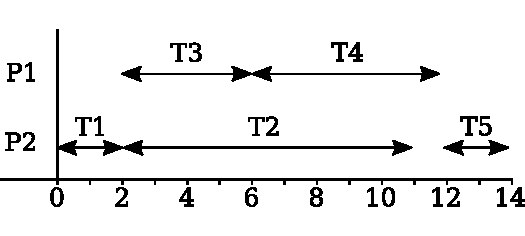
\includegraphics[width=0.45\columnwidth]{schedule.pdf}
    }
    \caption{A example of task graph scheduling}
    \label{fig:example}
\end{figure}

To enable a bog task for paralleled execution, a common way is to divide the original task into small tasks, then distribute the sub-tasks to several processors. If the task is infinitely separable, using this method reduces the total time by a factor of n, where n is the amount of processors. For real-time systems, it also means reduction in delay. However, in many of cases, some sub-tasks have to be executed in certain order, or called dependency. Such relationship can be represented by a task graph.

Figure \ref{fig:graph} shows an example of task graph, where each task is described in the format of ``identifier (duration)'' and dependencies are given as arrows pointing to dependant. An arrow pointing from task A to task B means task A have to be finished before the start of task B. Figure \ref{fig:schedule} shows an example schedule using two processors P1 and P2, where lines with arrows shows that one processor is allocated to one task in given period. It can be observed that the schedule reduces total execution time from 23 units sequentially to 14 units. In most of schedules, processors can not be made running during the entire period due to the dependencies, so that scheduling algorithms are used to better utilize the processors.

The complexity of this topic is the variation of models. The model given in figure \ref{fig:example} is based on the simplest assumption: each task takes same time on different processors and data can be distributed to other processors immediately. However, to better describe practical tasks, models are given more details. Here are several well-developed variances of models:

\begin{itemize}
    \item Homogeneous vs.\ heterogeneous in performance of each processor: For homogeneous clusters, the processors are considered to be equally powerful. For heterogeneous clusters \cite{Topcuoglu}, a simple model is to have different multipliers for each processor, making some of them faster to finish one task compared to other processors. In addition, complex models can include specialized processors in the cluster, usually related to specialized instruction sets or usage of co-processors, making them faster only for certain types of tasks. 
    \item Ideal (immediate) vs.\ practical in communication performance: For ideal situation, it is considered to happen immediately to transfer data from one processor to another, while it can take some time in practical models. With more details, the time consumption of communication can also depend on the size of messages. In this case the algorithms have to consider size of messages between each tasks due to the difference in time delay.
    \item Multiple vs.\ single communication channel in each processor: For models assuming multiple communication channels, each processor can communicate with many processors simultaneously, while it is considered to be able to send or receive data from only one processor in models assuming single communication channel.
\end{itemize}

There are also variances in scheduling algorithms. For the well discussed algorithm, list scheduling algorithm, different functions can be used to determine the priority of tasks, such as longest path, longest time and critical path, which can have significant effect to allocation results. This project will try to cover all the variances described above.

\subsection{Education Software}

There are many projects trying to develop applications for teaching assistance, for topics including algorithms, data structures or more complex concepts like programming. Shabanah et al.\ developed several applications to introduce basic algorithms like binary search and data structures like linked list and binary search tree\cite{Shabanah2010}. The robot game Karel is used by many universities to teach programming, especially for ideas related to sequence control, making the learning process more enjoyable\cite{Becker2001}. In addition, Harteveld et al. reviewed 36 projects for similar purposes \cite{Harteveld}.

There are more games designed based on engineering tasks. The game company Zachtronics is famous for such games. For example, ``TIS-300'' is designed based on the model with a mixture of assembly programming and manycore parallelism and ``Infinityfactory'' is designed based on production line management and geometric relationships. In addition, the game ``Screeps'' uses Javascript, a widely used programming language, as the main method to play the game, by programming AI of entities in the in-game world, for which the game is also suggested as a tool to learn programing.

\section{Programme and Methodology}

\subsection{Learning experience} \label{sec:modes}

This applications is expected to provide a complete description of different scenarios of task graph scheduling. For example, static systems are required to be optimized for only one task graph, but for dynamic systems, the have to adapt to changes in task graphs or to discover new tasks in real-time, which could lead to difference in preferred allocation. Therefore, it is designed to have different modes for different purposes:

\begin{enumerate}
    \item \textbf{Static:} The user is required to discover a schedule with requirements like total time or utilization rate, base on one fixed task graph. There is no time limit.
    \item \textbf{Dynamic:} The user is required to schedule and finish all the tasks from a dynamically expanding task graph. The processors will run in real time and the task graph will be gradually revealed. So the user have to determine the allocation quickly.
    \item \textbf{Leaning:} The user is required to provide the schedules generated by existing algorithms. The application will provide instructions to learn the algorithms and check if the provided schedule matches the expected one.
    \item \textbf{Multiplayer:} Similar to dynamic mode, but multiple players are competing to finish the tasks in shortest time.
    \item \textbf{Testing:} The user can develop a scheduling algorithm (possibly in Java), then the application will run the algorithm and show the result.
\end{enumerate}

Some modes like static mode and dynamic mode seems simple to implement, while modes like testing mode seems challenging, especially when letting the user to write programs inside the application. Therefore, testing mode will be implemented only if time allows, while other modes are expected to be finished.

\subsection{Appearance} \label{sec:aprc}

There are many choices to be made in design of this project. An important part is the design of the interface. The main idea is to provide intuitive interaction and representation of the task. For example, the user should be able to use drag and drop to allocate tasks to processors. For tasks, there can be many representations, which is given in figure \ref{fig:repr} and table \ref{tab:repr}, according to the task graph given in figure \ref{fig:graph}. In design of games, text are usually avoided because 1) it takes more effort for human to read compared to shapes and 2) text is more complex in layout of interface, especially when considering localization. Figure \ref{fig:repr} is made according to this design logic, using rectangles for tasks with solid squares for duration. Table \ref{tab:repr} shows the same information using a more formatted structure. It is easy to be read by machine and stored in database, but for human, it is more difficult to recognize the dependencies. There can be more formats to represent the same structure, but in a game-like application, formats similar to figure \ref{fig:repr} are more likely to be used.

\begin{figure}
\begin{minipage}{\textwidth}
    \vspace{1em}
    \hfill
    \begin{minipage}[b]{0.4\textwidth}
        \centering
        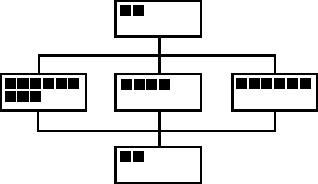
\includegraphics[width=0.7\textwidth]{repr.pdf}
        \vspace{0.5em}
        \captionof{figure}{A representation of\\ task graph using shapes}
        \label{fig:repr}
    \end{minipage}
    \hfill
    \begin{minipage}[b]{0.49\textwidth}
        \center
        \begin{tabular}{ccc}\hline
            Identifier & Duration & Dependencies \\ \hline
            task 1 & 2 units &  \\
            task 2 & 9 units & task 1 \\
            task 3 & 4 units & task 1 \\
            task 4 & 6 units & task 1\\
            task 5 & 2 units & task 2, 3, 4 \\ \hline
        \end{tabular}
        \captionof{table}{A representation of\\ task graph using one table}
        \label{tab:repr}
    \end{minipage}
    \hfill
    \vspace{1em}
\end{minipage}
\end{figure}

In addition to details, the quality of layout also contributes to the overall usability. Figure \ref{fig:layout} shows an typical layout of interface, showing task graph on the left side, status of processors on the right side and allocation of tasks in the bottom. One possible method to represent task allocation is to have several rows, each for one processor, to show the timeline of processors, so that the user can drag and drop tasks into the timeline of any processor with results shown in real-time. There can be many choices in layout, but it should provide significant amount of information to the user.

\begin{figure}[htpb]
    \centering
    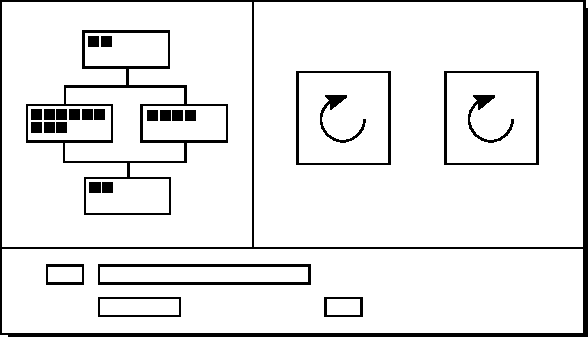
\includegraphics[width=0.5\columnwidth]{layout.pdf}
    \caption{A example layout of interface}
    \label{fig:layout}
\end{figure}

\subsection{Implementation}

To provide simplicity in usage and accessability in different environments, the application is decided to be a cross-platform native application. There are many options to build a cross-platform application like 1) write the program in C++ and cross compile to different platforms, 2) write the program in Java (or other JVM languages) and use dedicated virtual machine on different platforms and 3) write the program in Python or other scripting language and use different interpreter on different platforms. The final choice is to use Java because it provides a balance in performance and simplicity of development. Although installation of Java virtual machine is sometimes annoying, considering the application is intended to be used on DICE \footnote{DICE: the computing platform of university base on Linux with Java 8 installed by default} machines and by computer science students, it should be relatively easy to setup.

As is described in section \ref{sec:aprc}, this program might require usage of textures and animations, which is not emphasized in traditional GUI \footnote{GUI: graphical user interface} frameworks. Although there are several well known GUI frameworks in Java like AWT, Swing and JavaFx, the final choice is to build a dedicate GUI framework to provide more flexibility and consistency on different platforms, similar to many games. There are several low-level libraries or game engines to build an application with customized rendering, including libGDX, jMonkeyEngine and LWJGL. The final choice is to use LWJGL because 1) it has great community support; 2) it provides full exposure of native interfaces of OpenGL -- a cross-platform graphical API \footnote{API: application programming interface} and 3) it contains handy support for other parts in application development like audio playback.

\section{Evaluation} \label{sec:eva}

This project will mainly be evaluated in two aspects: quality of design, which is more important, and quality of implementation. Since the application is developed for education purpose, the design will be evaluated according to learning results of testers. Although there are some arguments, the application will be tested base on five user assumption \cite{Virzi1992}, due to the limit of time. According to the assumption, 5 students will be invited to use the application to learn task graph scheduling algorithms. The testers will be suggested to continuously describe their thoughts about the experience, so that the entire process can be recorded. Afterwards, the testers will be asked some questions to evaluate their understanding of the algorithms. Ideally, the users are expected to know variances described in section \ref{sec:tgs} and tell the detailed execution of algorithms in different models.

The process is expected to take less than 4 hours, because it will become hard to arrange if it takes longer. The duration seems not sufficient for a student to understand all the details of the algorithms. In this case, if the tester is willing to, he/she can copy the application for further study and provide more feedback on user experience.

For quality of implementation, it will be evaluated according to compatibility in different environments like variant operating systems, hardware configurations and screen resolution. It should at least run successfully out-of-box on DICE machines and is highly expected to run correctly on Linux and Windows. In addition, criterions like quality of documentation and program structure will be discussed.

\section{Expected Outcomes}

Since this project is mainly development based, the main outcome is the compiled executable and source code of the application. For testing mode described in section \ref{sec:modes}, there will be brief documentation if it requires extra steps to setup. In addition, test results described in section \ref{sec:eva} will be given. As described in previous sections, this application is expected to improve efficiency of learning. It is also important to provide interesting and satisfying learning experience because it makes the students willing to study.

\section{Research Plan, Milestones and Deliverables}

% \definecolor{barblue}{RGB}{153,204,254}
% \definecolor{groupblue}{RGB}{51,102,254}
% \definecolor{linkred}{RGB}{165,0,33} 

% \begin{figure}[htbp]
% \begin{ganttchart}[
%     y unit title=0.4cm,
%     y unit chart=0.5cm,
%     vgrid,hgrid,
%     x unit=1.55mm,
%     time slot format=isodate,
%     title/.append style={draw=none, fill=barblue},
%     title label font=\sffamily\bfseries\color{white},
%     title label node/.append style={below=-1.6ex},
%     title left shift=.05,
%     title right shift=-.05,
%     title height=1,
%     bar/.append style={draw=none, fill=groupblue},
%     bar height=.6,
%     bar label font=\normalsize\color{black!50},
%     group right shift=0,
%     group top shift=.6,
%     group height=.3,
%     group peaks height=.2,
%     bar incomplete/.append style={fill=green}
%    ]{2018-06-01}{2018-08-16}
%    \gantttitlecalendar{month=name}\\
%    \ganttbar[
%     progress=100,
%     bar progress label font=\small\color{barblue},
%     bar progress label node/.append style={right=4pt},
%     bar label font=\normalsize\color{barblue},
%     name=pp
%    ]{Background Reading}{2018-06-01}{2018-06-14} \\
% \ganttset{progress label text={}, link/.style={black, -to}}
% \ganttgroup{Objective 1}{2018-06-14}{2018-06-30} \\
% \ganttbar[progress=4, name=T1A]{Task A}{2018-06-14}{2018-06-21} \\
% \ganttlinkedbar[progress=0]{Task B}{2018-06-21}{2018-06-30} \\
% \ganttgroup{Objective 2}{2018-07-01}{2018-07-14} \\
% \ganttbar[progress=15, name=T2A]{Task A}{2018-07-01}{2018-07-07} \\
% \ganttlinkedbar[progress=0]{Task B}{2018-07-07}{2018-07-14} \\
% \ganttgroup{Dissertation    }{2018-07-14}{2018-08-16} \\
%   \ganttbar[progress=0]{Task A}{2018-07-14}{2018-08-16}
%   \ganttset{link/.style={green}}
%   \ganttlink[link mid=.4]{pp}{T1A}
%   \ganttlink[link mid=.159]{pp}{T2A}
% \end{ganttchart}
% \caption{Gantt Chart of the activities defined for this project.}
% \label{fig:gantt}
% \end{figure}

\begin{table}[htbp]
    \begin{center}
        \begin{tabular}{|c|c|l|}
        \hline
        \textbf{Milestone} & \textbf{Week} & \textbf{Description} \\
        \hline
        $M_1$ & 2 & Building blocks and utilities completed \\
        $M_2$ & 5 & Static, dynamic and learning mode completed \\
        $M_3$ & 8 & Multiplayer and testing mode completed \\
        $M_4$ & 9 & Testing completed \\
        $M_5$ & 10 & Submission of dissertation \\
        \hline
        \end{tabular} 
    \end{center}
    \caption{Milestones defined in this project.}
    \label{fig:milestones}
\end{table}

% \begin{table}[htbp]
%     \begin{center}
%         \begin{tabular}{|c|c|l|}
%         \hline
%         \textbf{Deliverable} & \textbf{Week} & \textbf{Description} \\
%         \hline
%         $D_1$ & 6 & Software tool for \dots\\
%         $D_2$ & 8 & Evaluation report on \dots\\
%         $D_3$ & 10 & Dissertation \\
%         \hline
%         \end{tabular} 
%     \end{center}
%     \caption{List of deliverables defined in this project.}
%     \label{fig:deliverables}
% \end{table}


%                Now build the reference list
\FloatBarrier
\bibliographystyle{unsrt}   % The reference style
%                This is plain and unsorted, so in the order
%                they appear in the document.

{\small
\bibliography{main}       % bib file(s).
}
\end{document}

